\chapter{Concepts}
\section{Jupiter}
\emph{Jupiter} is a collaboration system that supports shared documents, shared tools, and, optionally, live audio/video communication. It was developed by \emph{Xerox}. It is conceptually a collaborative windowing toolkit. The low-level communication facilities are based on operational transformation.

The operational transformation algorithm employed in the \emph{Jupiter} system is derived from \emph{dOPT}. A centralized architecture and thus the reduction to point-to-point connections makes the algorithm significantly simpler than other operational transformation algorithms. The basic \emph{Jupiter} algorithm is only suitable for two sites. However, it was shown in \cite{jupiter95} and in greater detail in \cite{netedit:thesis} how to use several point-to-point connections to build a tree-structured $n$-site algorithm (see figure \ref{fig:concepts.nway}).

\begin{figure}[htb]
 \centering
 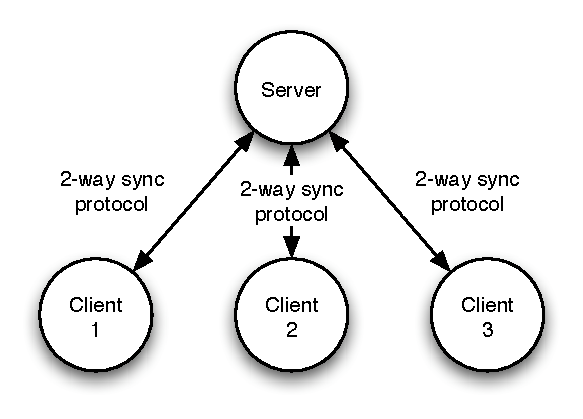
\includegraphics[width=9.3cm,height=6.5cm]{../../images/concepts_nway.eps}
 \caption{Multiple 2-way Sync to Achieve n-way Sync}
 \label{fig:concepts.nway}
\end{figure}

\subsection{Algorithm}
The general tool for handling conflicting (i.e. concurrent) requests is the transformation function, called $xform$ in \cite{jupiter95}.

$$ xform(c,s)=\{c',s'\} $$

This transformation function takes two requests, $c$ from the client and $s$ from the server, and returns two transformed requests $c'$ and $s'$. The requests $c'$ and $s'$ have the property that if the client applies $c$ followed by $s'$, and the server applies $s$ followed by $c'$, both client and server wind up in the same final state (see figure \ref{fig:concepts.basic}). This property is also known as transformation property 1 (TP1):

$$ c s' \equiv s c' $$

\begin{figure}[htb]
 \centering
 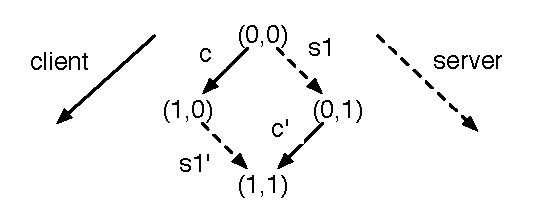
\includegraphics[width=8.5cm,height=3.1cm]{../../images/concepts_jupiter1.eps}
 \caption{Basic Transformation Situation in Jupiter}
 \label{fig:concepts.basic}
\end{figure}

Conceptually, the $xform$ function is a combined inclusion transformation (IT) that returns $\{IT(c,s),IT(s,c)\}$.

\subsubsection{State Space Graph}
As we have seen, it is helpful to show the two dimensional state space that both client and server pass through as they process requests (see figure \ref{fig:concepts.statespace}). Each state is labelled with the number of processed requests from both client and server to that point. For instance if the client is in the state $(2,3)$, it has generated and processed two requests of its own, and has received and processed three from the server. The client and server requests are displayed on different axis in the state space graph.

\begin{figure}[htb]
 \centering
 \includegraphics[width=8.4cm,height=5.7cm]{../../images/concepts_statespace.eps}
 \caption{Two Dimensional State Space Example}
 \label{fig:concepts.statespace}
\end{figure}

If there is a conflict, the paths will diverge, as shown in figure \ref{fig:concepts.statespace}. The client and server moved to the state $(1,1)$ together by first processing a client request, and then a server request. At that point, the client and server processed different requests (concurrently), moving to state $(2,1)$ and $(1,2)$ respectively. They each received and processed the other's message using the transformation function to move to state $(2,2)$.

The algorithm labels each request with the state the sender was in just before the message was generated (state vector). The recipient uses these labels to insert the request into his state space. If the request does not start from the current state the recipient is in, there is a conflict (concurrent request). Two concurrent requests have to be transformed, but they can only be transformed directly when they were generated from the same state of the document.

If client and server diverge more than one step in the state space graph, the transformation function cannot be applied directly. Let us consider the state space in figure \ref{fig:concepts.statespace2}. The client has executed $c$ and receives the conflicting request $s1$ from the server. It uses the transformation function to computer $s1'$ to get to the state $(1,1)$. The server then generates $s2$ from the state $(0,1)$, indicating that it still has not processed $c$. What should the client do now? It cannot use the transformation function directly because $c$ and $s2$ were not generated from the same document state.

\begin{figure}[htb]
 \centering
 \includegraphics[width=8.5cm,height=5.7cm]{../../images/concepts_statespace2.eps}
 \caption{Client and Server Diverging by more than one Path Step}
 \label{fig:concepts.statespace2}
\end{figure}

The solution to this situation is as follows. When the client computes $s1'$ it must also remember $c'$. This represents a hypothetical request that the client could have generated to move from the state $(0,1)$ to $(1,1)$. When $s2$ arrives, the client can user $c'$ to compute $c''$. It executes $s2'$ to get to the state $(1,2)$. If the server has processed the client's message, it will be in the state $(1,2)$ as well. If not, its next request will originate from $(0,3)$, so the client saves $c''$ just in case.

The algorithm guarantees that if the transformation function satisfies TP1, then no matter how far the client and server diverge in state space, when they do reach the same state, they will have equivalent states (so convergence is achieved).

\subsubsection{Extending Jupiter to N-Way Communication}
We have discussed how a single two-way connection works in \emph{Jupiter}. We will now extend this systems to support $n$ clients using multiple two-way connections. The figure \ref{fig:concepts.nway-details} shows the basic setup for three clients. Each client talks only to the server over a standard well-knwon two-way connection. On the server, there is one so-called client proxy per client. This client proxy conceptually is just the server side algorithm. 

\begin{figure}[htb]
 \centering
 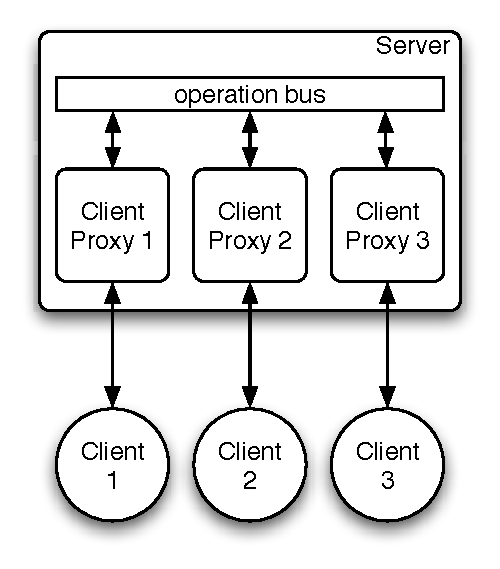
\includegraphics[width=7.9cm,height=9.06cm]{../../images/concepts_nway-details.eps}
 \caption{N-Way Synchronization using Central Server}
 \label{fig:concepts.nway-details}
\end{figure}

When a client sends a request to the server, the corresponding client proxy algorithm transforms the request against any concurrent requests the server already sent to the client but that were not acknowledged by the client. This client proxy then dispatches the operation to all other client proxies (over a operation bus). The other client proxies get this operation from the operation bus and insert it into their algorithm as local operation. The resulting request is then sent to the client the client proxy represents. 

One thing must be taken care of in the implementation. Only one request may be processed by the server at any time. That is, the processing of requests from clients must be serialized. Otherwise, the algorithm will not work correctly.

\paragraph{n-way Example:} In order to better understand how the n-way synchronization work, we examine a simple example. In figure \ref{fig:concepts.nway-example-1}, the bottom two state graphs represent two clients, the top two state graphs represent the server, or more exactly the client proxy algorithms on the server. 

In the first step, both clients generate a request and send it to the server (see figure \ref{fig:concepts.nway-example-1}). Then the request from client 1 arrives at the server earlier than the request from client 2 and is therefore processed first (see figure \ref{fig:concepts.nway-example-2}). In the next step, the request from client 2 is processed by the server (see figure \ref{fig:concepts.nway-example-3}). In the last step both clients receive the transformed request from their corresponding client proxy on the server side (see figure \ref{fig:concepts.nway-example-4}). They insert the requests at the right positions in their state space, doing transformations as necessary (client 2 has to transform the incoming message, client 1 not).

\begin{figure}[H]
 \centering
 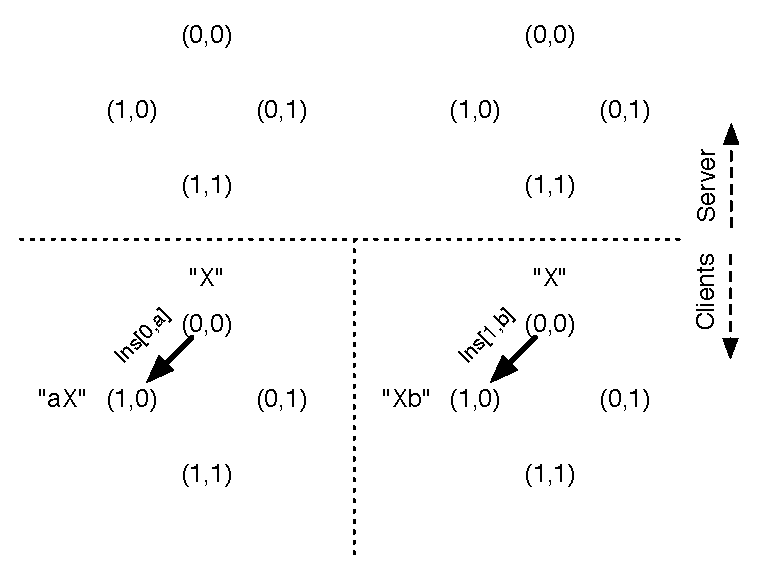
\includegraphics[width=10.0cm,height=7.54cm]{../../images/concepts_nway-example-1.eps}
 \caption{n-way example (step 1)}
 \label{fig:concepts.nway-example-1}
\end{figure}

\begin{figure}[H]
 \centering
 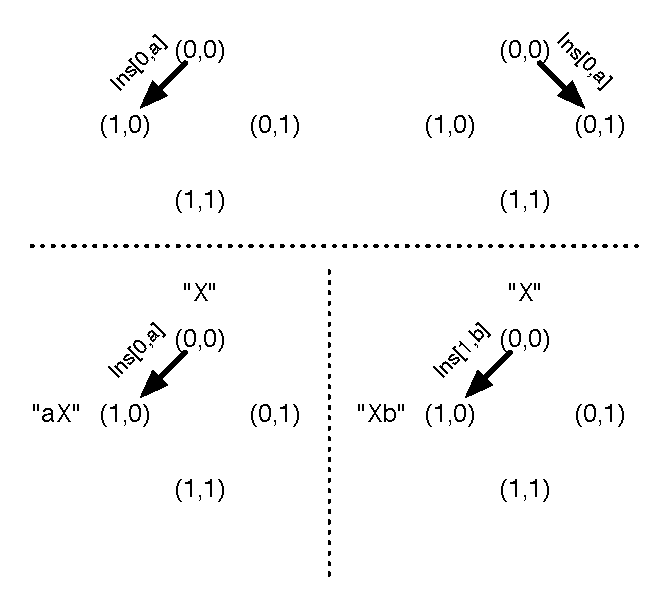
\includegraphics[width=10.0cm,height=7.74cm]{../../images/concepts_nway-example-2.eps}
 \caption{n-way example (step 2)}
 \label{fig:concepts.nway-example-2}
\end{figure}

\begin{figure}[H]
 \centering
 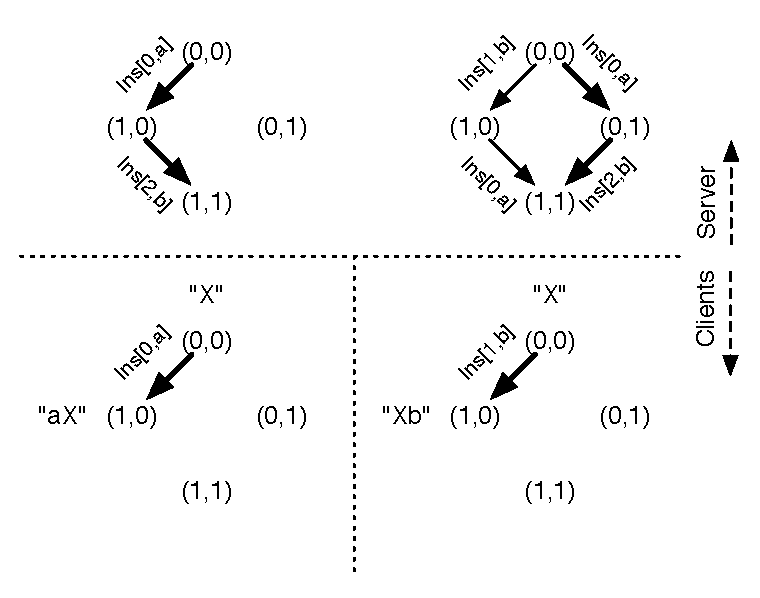
\includegraphics[width=10.0cm,height=7.77cm]{../../images/concepts_nway-example-3.eps}
 \caption{n-way example (step 3)}
 \label{fig:concepts.nway-example-3}
\end{figure}

\begin{figure}[H]
 \centering
 \includegraphics[width=10.0cm,height=7.77cm]{../../images/concepts_nway-example-4.eps}
 \caption{n-way example (step 4)}
 \label{fig:concepts.nway-example-4}
\end{figure}


\subsection{Undo/Redo}
In the preceeding sections, we have presented the basic transformation algorithm. In this section we will show how undo/redo of local operations can be achieved in a real-time collaborative editor. This introduces a whole set of new problems that necessitate additions to the transformation algorithm.

\subsubsection{Problems of Local Group Undo}
Global group undo is not much different from common single-user undo schemes. It can be implemented by executing the inverse command for each user command to be undone. The operation to be undone is the globally last operation that was executed. Global undo always leads to a former application state. In contrast, local group undo (undoing the last operation from the local user) is more complex, because in most cases it does not lead to a former application state.

\paragraph{Example 1:} Suppose the initial document state is 'm'. Now user $X$ executes the command $Ins[1,'s']$ to insert the character 's' at position 1 of the document. Then user $Y$ executes $Ins[1,'a']$ to insert the character 'a' at position 1 resulting in a document state 'mas'. Now user $X$ decides to undo his last insertion command. What has to be done? The naive, but incorrect approach would just execute $Del[1,'s']$, i.e. the inverse to $Ins[1,'s']$. However, the current character at position 1 is not 's' but 'a'. The situation is depicted in figure \ref{fig:concepts.naiveundo}.

\begin{figure}[htb]
 \centering
 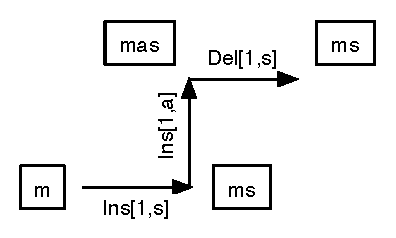
\includegraphics[width=6.13cm,height=3.45cm]{../../images/concepts_naiveundo.eps}
 \caption{Incorrect Naive Approach to Local Group Undo}
 \label{fig:concepts.naiveundo}
\end{figure}

Obviously, just executing the inverse of the last local operation cannot achieve the correct result. In addition, there are more situations were local group undo methods can fail. One characteristic example is the following problem, which is called \emph{order puzzle}.

\paragraph{Example 2:}
Suppose we start with a document containing 'ab'. Now user 'X' first deletes 'a' by executing $Del[1,'a']$. Afterwards user $Y$ deletes 'b' by issuing the command $Del[1,'b']$. This will leave the document empty. Now both users undo their commands. The expected application state should be 'ab' afterwards, because undoing all commands should not modify the original application state. Unfortunately, a naive undo solution could yield the wrong state 'ba'. The solution to the order puzzle will be presented in a later section.

\subsubsection{Transformation-Based Local Group Undo}
Let us return to the example 1. Suppose we want to undo the last command after a command from another participant has already been executed. For correctness of local group undo, we required that the effect of the undo request does not depend on other users' requests. Therefore, we may safely assume, that we issued the undo command immediately after the execution of the command wot be undone. Then the appropriate transformations can be applied to gain the command that has to be executed in the present state. 

In example 1, we insert the inverse operation $Del[1,'s']$ immediately after the operation. The procedure of inserting the inverse operation is called \emph{mirroring}. In the next step, the inverse operation $Del[1,'s']$ is transformed against the operation $Ins[1,'a']$ from user $Y$, which results in the correct operation $Del[2,'s']$. See figure \ref{fig:concepts.undobytransformation}.

\begin{figure}[htb]
 \centering
 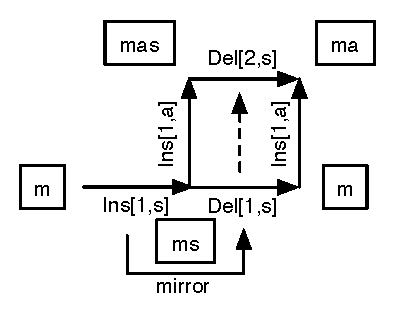
\includegraphics[width=6.13cm,height=4.79cm]{../../images/concepts_undobytransformation.eps}
 \caption{Local Undo by Transformation}
 \label{fig:concepts.undobytransformation}
\end{figure}

Unfortunately, the computation of requests in the interaction model by transformation and by mirroring is not sufficient to solve the \emph{order puzzle} in example 2.

\paragraph{Example 3:} Suppose both users $X$ and $Y$ simultaneously delete the single character 'b' (see figure \ref{fig:concepts.basicfold}). The corresponding transformation rule transform both operations to noop operations, since deleting the same character twice is impossible. Now suppose, user $Y$ wants to undo his command $Del[0,'b']$. We know this can be achieved by applying the mirror operator, adding the command $Ins[0,'b']$. Now, how can the missing commands be computer? By just applying the transformation rule, the commands would just be copied without modification, e.g., another noop command would lead from state 'b' to the end state 'b' (in the upper right corner). However, this violates the principle of correctness, namely that a set of do-undo pairs like $Del[0,'b']$ and $Ins[0,'b']$ should have no effect on other users' commands. If this were to be satisfied, the resulting state should be empty, as after just executing user X's command $Del[0,'b']$. 

\begin{figure}[htb]
 \centering
 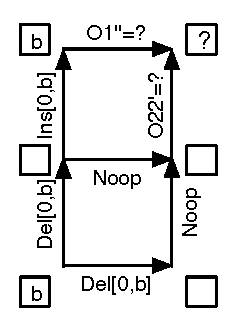
\includegraphics[width=3.45cm,height=4.97cm]{../../images/concepts_basicfold.eps}
 \caption{Application of Mirror and Fold Operators}
 \label{fig:concepts.basicfold}
\end{figure}


\subsubsection{Fold Operator}
To solve the puzzle in example 3, we observer that all parallel lines connected by do-undo pairs should actually contain congruent requests and states. Here in the example $O_{1}''$ should be $Del[0,'b']$, and the resulting state should be empty, like the command and the state at the bottom of the diagram (see figure \ref{fig:concepts.basicfold}).

We denote the copying of a request from the beginning of a do-undo pair - or more general a set of possibly nested do-undo pairs - to the end of the do-undo pair as \emph{folding}. This illustrates the fact that we might actually fold the interaction model - here along the straight line defined by the horizontal noop request in the center - so that both planes come to lie above each other. 

To complete the interaction model correctly we demand that $O_{22}'$ will be computed by mirroring the operation noop (in figure \ref{fig:concepts.basicfold} at the bottom right). The resulting interaction model with all mirror and fold operators applied is displayed in figure \ref{fig:concepts.basicfold-solution}.

\begin{figure}[htb]
 \centering
 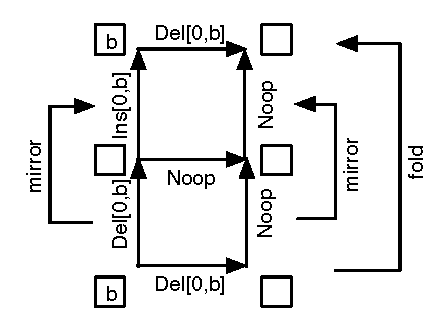
\includegraphics[width=6.99cm,height=4.97cm]{../../images/concepts_basicfold-solution.eps}
 \caption{Application of Mirror and Fold Operators}
 \label{fig:concepts.basicfold-solution}
\end{figure}


\subsubsection{Solution to the Order Puzzle}
The solution to the order puzzle in example 2 can be computed with the same operators, mirror and fold. The desired result is shown in figure \ref{fig:concepts.orderpuzzle}.

\begin{figure}[htb]
 \centering
 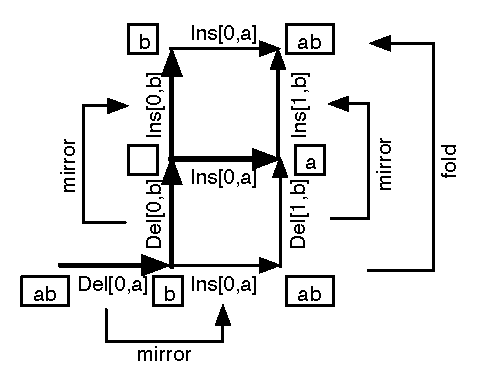
\includegraphics[width=7.55cm,height=5.96cm]{../../images/concepts_orderpuzzle.eps}
 \caption{Solution to the Order Puzzle}
 \label{fig:concepts.orderpuzzle}
\end{figure}


\subsubsection{Additional Problems in n-Way Situation}
Unfortunately, there exists another problem in the n-way situation that do not exist in the 2-way situation. To illustrate the problem and the solution we introduce another example.

\paragraph{Example 4:} First, user $X$ generates the request $Del[0,b]$ from the initial document state 'b'. Then, he undoes that change immediately (generating the mirror request $Ins[0,b]$). User $Y$ generates the request $Del[0,b]$ concurrently to the two requests from user $X$ (see figure \ref{fig:concepts.transformation-history-1}). In figure \ref{fig:concepts.transformation-history-2} the first request from user $X$ is processed by the server and then by the user $Y$. Nothing unusual happens in this situation. Then the request from user $Y$ is processed by the server, resulting in a Noop operation (see figure \ref{fig:concepts.transformation-history-3}).

The next step (see figure \ref{fig:concepts.transformation-history-4}) reveals the interesting problem. The Noop operation is inserted into the state space of user $X$. Now we need to calculate operation $O_{x}$. Because the Noop operation is between a do-undo pair (mirror), $O_{x}$ must be calculated by folding the state space graph, that is by putting the dashed operation $O_{x}$ from the bottom to the top line. The problem is, we do not know what this operation was, so we cannot apply the fold operator.

In figure \ref{fig:concepts.transformation-history-5} we see a similar problem on the server-side, or more specifically at the client proxy of user $X$ at the server. Here, the undo request from user $X$ has arrived at the server and is inserted into the state space graph at the correct position (from $(0,1)$ to $(0,2)$). Because we have a do-undo pair (mirror) on the bottom line, we must have a mirror operation on the second line too according to our transformation rules. In order to calculate $O_{y}$ we need to know the operation marked with three question marks first. This operation can be calculated by transforming $Del[0,b]$ against $O_{x}$. Once again, this operation is missing.

So how do we find out $O_{x}$? The answer lies in the fact that the Noop request resulted from a transformation, so $O_{x}$ was known by the client proxy of user $Y$. It is $Del[0,b]$. If we remember the transformation history of an operation, we can use these previous forms of an operation to successfully apply mirror and fold operators and thus solve the problem presented in this example.

\begin{figure}[H]
 \centering
 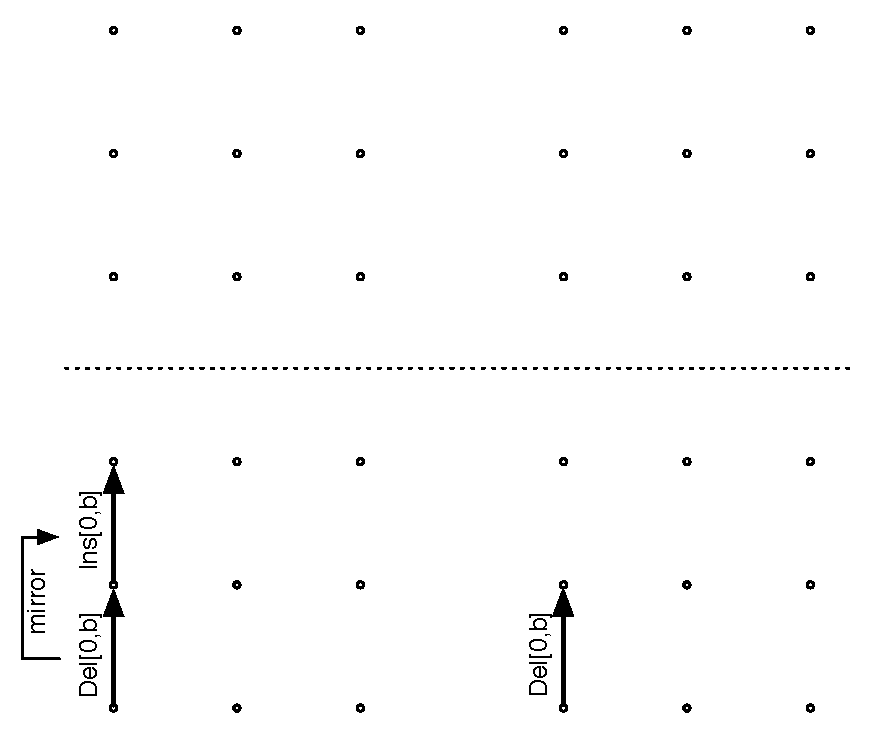
\includegraphics[width=10cm,height=8.36cm]{../../images/concepts_transformation-history-1.eps}
 \caption{n-way undo problem (step 1)}
 \label{fig:concepts.transformation-history-1}
\end{figure}

\begin{figure}[H]
 \centering
 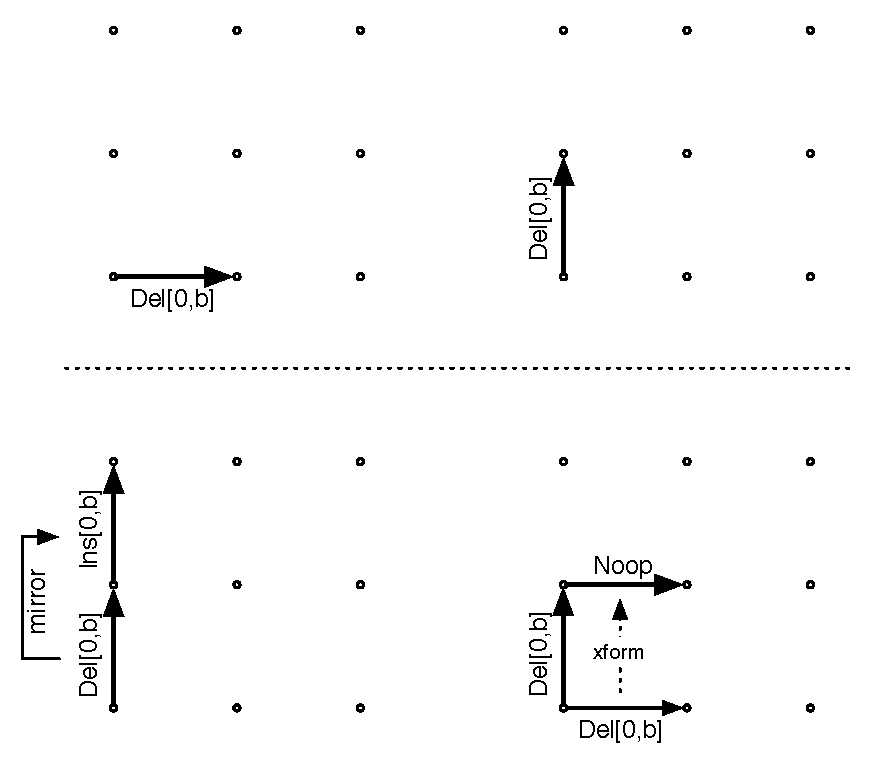
\includegraphics[width=10cm,height=8.69cm]{../../images/concepts_transformation-history-2.eps}
 \caption{n-way undo problem (step 2)}
 \label{fig:concepts.transformation-history-2}
\end{figure}

\begin{figure}[H]
 \centering
 \includegraphics[width=10cm,height=8.69cm]{../../images/concepts_transformation-history-3.eps}
 \caption{n-way undo problem (step 3)}
 \label{fig:concepts.transformation-history-3}
\end{figure}

\begin{figure}[H]
 \centering
 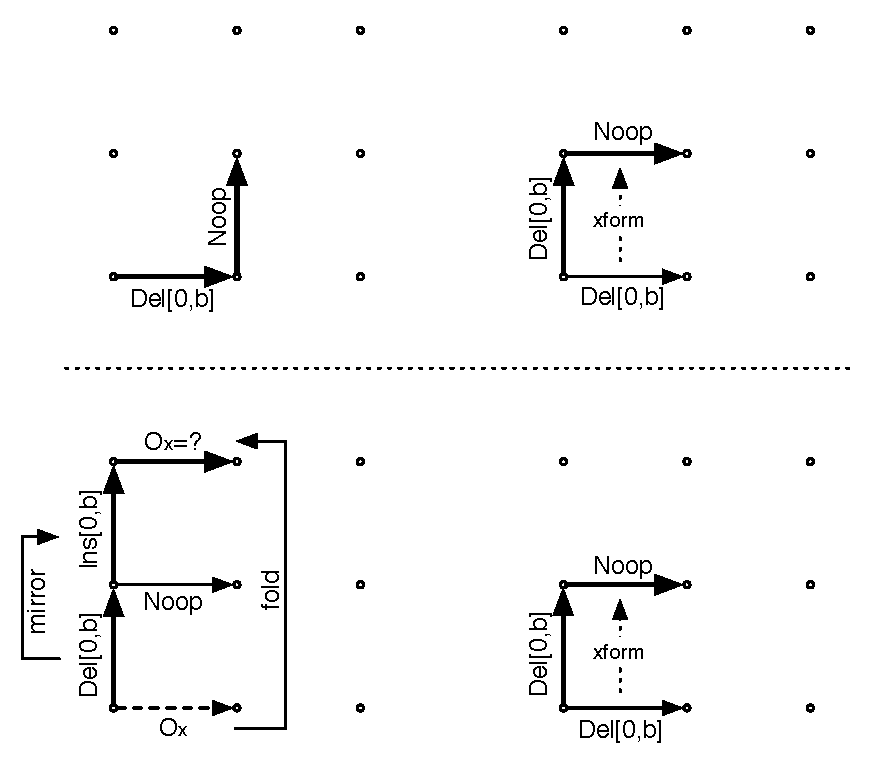
\includegraphics[width=10cm,height=8.69cm]{../../images/concepts_transformation-history-4.eps}
 \caption{n-way undo problem (step 4)}
 \label{fig:concepts.transformation-history-4}
\end{figure}

\begin{figure}[H]
 \centering
 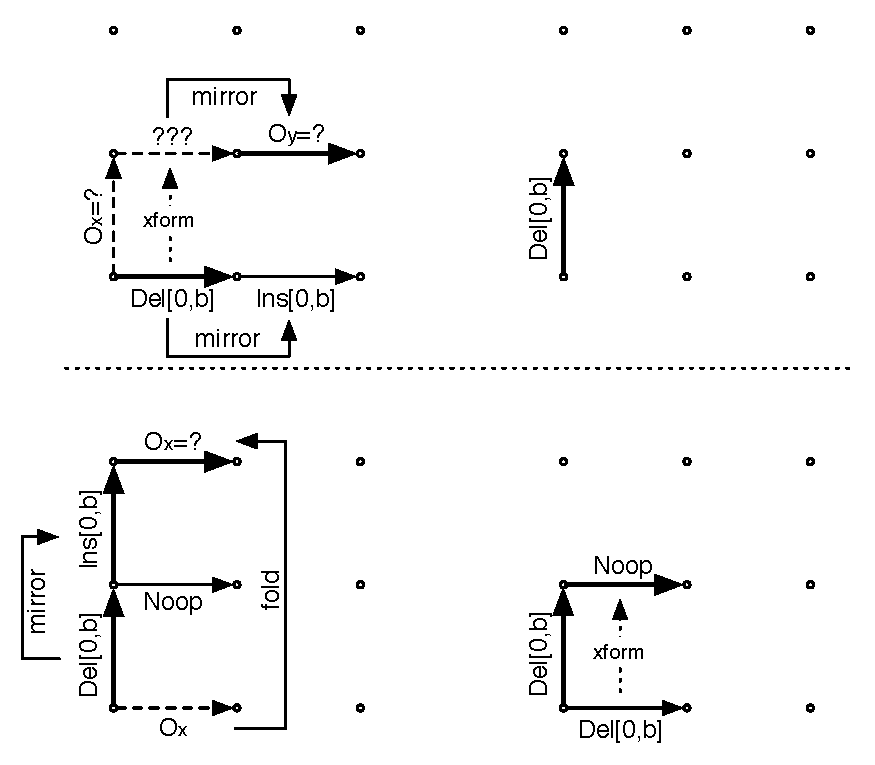
\includegraphics[width=10cm,height=8.69cm]{../../images/concepts_transformation-history-5.eps}
 \caption{n-way undo problem (step 5)}
 \label{fig:concepts.transformation-history-5}
\end{figure}


\subsubsection{Redo}
The integration of a redo operation has never been considered before in the area of operational transformation algorithms. However, it turned out to be rather straightforward to implement a redo feature. A redo can only be done, if the last operation from a user has been an undo or there are only undo-redo pairs between the current state and an undo operation. A do operation between the current state and an undo operation effectively disables the redo (this is the normal behavior in any modern text processing application).

\begin{figure}[htb]
 \centering
 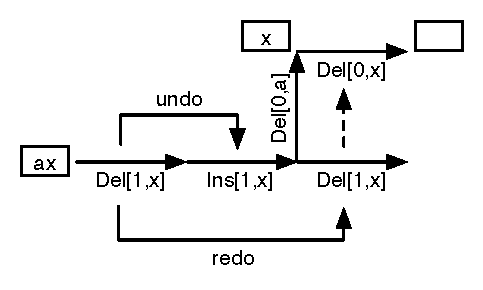
\includegraphics[width=7.62cm,height=4.34cm]{../../images/concepts_redo.eps}
 \caption{Redo Operation}
 \label{fig:concepts.redo}
\end{figure}

In figure \ref{fig:concepts.redo} we see how a redo is inserted into the state space. First, the last operation from this user must be a redo (or there are only undo-redo pairs between the current state and an undo operation). This is clearly the case in this example. We then copy the corresponding do operation to the current column in the state space on the same line as the original operation. We then have to transform this copied operation to the current state (so that we can apply it). This basic algorithm is always applicable.
